\chapter{Luồng hoạt động và kiến trúc công cụ}
\label{chap:method}

Chương này sẽ trình bày quy trình phân tích mã nguồn cho ngôn ngữ lập trình Rust bao gồm xây dựng cây cú pháp trừu tượng, ánh xạ từ cây cú pháp trừu tượng sang đồ thị thuộc tính mã nguồn.
Chương này cũng sẽ đào sâu vào kiến trúc của công cụ, bao gồm các thành phần chính và tương tác giữa chúng.

% \section{Luồng hoạt động}
\section{Luồng hoạt động và cài đặt công cụ}

\begin{figure}[H]
	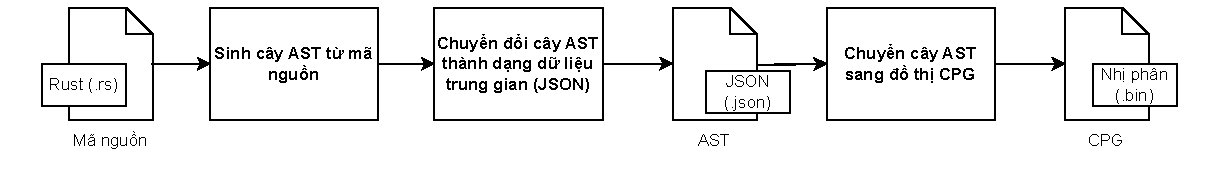
\includegraphics[width=1\columnwidth]{figures/c3/c3_flow_2.drawio.pdf}
	\centering
	\caption{Quy trình phân tích mã nguồn Rust.}
	\label{img:c3_flow_2}
\end{figure}

% \begin{figure}[H]
% 	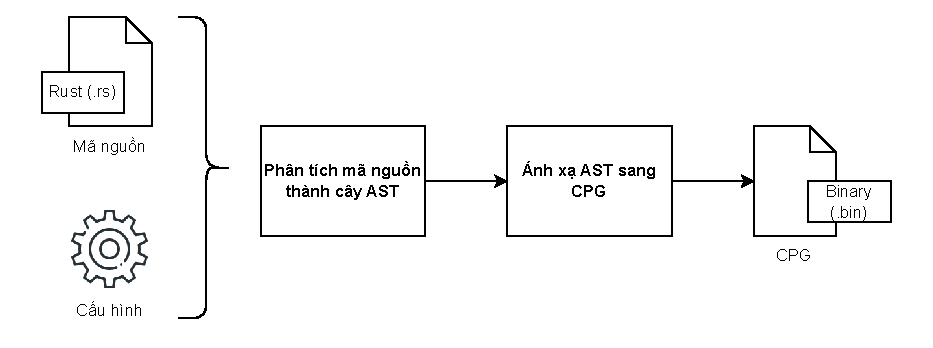
\includegraphics[width=1\columnwidth]{figures/c3/c3_flow.drawio.pdf}
% 	\centering
% 	\caption{Quy trình phân tích mã nguồn Rust.}
% 	\label{img:c3_flow}
% \end{figure}

% \begin{figure}[H]
% 	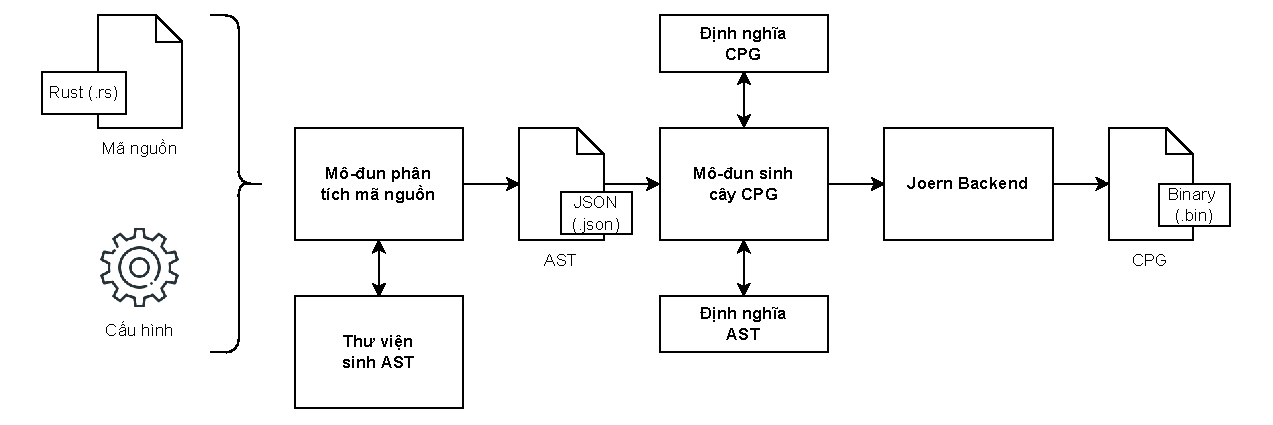
\includegraphics[width=1\columnwidth]{figures/c4/c4_install_flow.drawio.pdf}
% 	\centering
% 	\caption{Kiến trúc công cụ.}
% 	\label{img:c4_install_flow}
% \end{figure}

% \begin{figure}[H]
% 	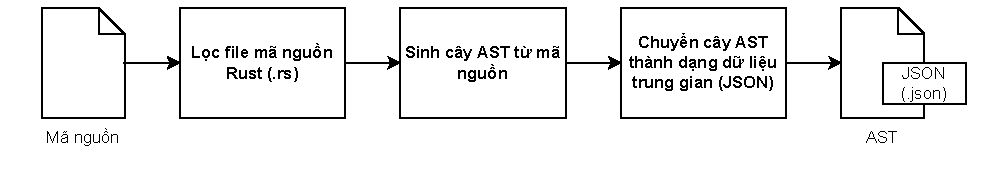
\includegraphics[width=1\columnwidth]{figures/c3/c3_flow_ast.drawio.pdf}
% 	\centering
% 	\caption{Quy trình xây dựng cây AST.}
% 	\label{img:c3_flow_ast}
% \end{figure}

Mục tiêu của công cụ là phân tích mã nguồn Rust và xây dựng đồ thị CPG biểu diễn mã nguồn đó.
% Đầu vào của công cụ là các tệp mã nguồn Rust, đầu ra là đồ thị CPG lưu dưới dạng nhị phân.
Đầu vào của công cụ là các tệp mã nguồn Rust, trong khi đầu ra là đồ thị CPG được lưu dưới dạng nhị phân để dễ dàng xử lý và lưu trữ.
Đồ thị CPG được phục vụ cho việc thực hiện các câu lệnh truy vấn trên đồ thị hoặc quét đồ thị để tìm lỗ hổng trong mã nguồn.
% Với yêu cầu đầu vào, đầu ra như trên, luồng hoạt động của công cụ bao gồm các bước được thể hiện trong hình \ref{img:c3_flow_2}.
Với yêu cầu đầu vào và đầu ra như trên, luồng hoạt động của công cụ được thiết kế thành các bước liên kết chặt chẽ và được thể hiện trong hình \ref{img:c3_flow_2}.
% Chi tiết các bước được tiến hành như sau:
% Các bước này bao gồm phân tích cú pháp mã nguồn, xây dựng cây AST, ánh xạ cây AST sang đồ thị CPG, và cuối cùng là xuất đồ thị dưới định dạng nhị phân.
Chi tiết các bước được tiến hành như sau:

\begin{enumerate}
	\item Từ thư mục của dự án, lọc lấy các tệp mã nguồn Rust (các tệp có đuôi \texttt{.rs}).
	\item Với mỗi tệp mã nguồn, sử dụng thư viện \textit{syn} \cite{synRust} để sinh cây AST từ nội dung mã nguồn của tệp đó.
	\textit{syn} là một thư viện phân tích mã nguồn thành cây AST được sử dụng rộng rãi với nhiều mục đích, trong đó bao gồm việc cài đặt tính năng Procedural Macro \cite{rustlangProceduralMacros} của Rust.
	Tính tới thời điểm hiện tại Rust không có đặc tả ngôn ngữ chính thức, do đó cộng đồng sử dụng Rust Reference \cite{rustReference} coi như phiên bản sát nhất so với một đặc tả ngôn ngữ.
	Thư viện syn xây dựng định nghĩa các nút của cây AST tuân theo Rust Reference.
	\item Chuyển đổi cây AST từ ngôn ngữ Rust sang định dạng JSON.
	Joern có thể được sử dụng cho nhiều ngôn ngữ và Joern Frontend không phụ thuộc vào bộ phân tích ngôn ngữ của một ngôn ngữ nhất định, do vậy cần có định dạng dữ liệu trung gian để chuyển đổi cây AST của bộ phân tích ngôn ngữ sang ngôn ngữ Scala của Joern Frontend.
	Có các kiểu dữ liệu trung gian phổ biến như JSON, XML, YAML, trong đó JSON được lựa chọn bởi tính đơn giản, dễ chuyển đổi.
	\item Cây AST dưới định dạng JSON được đọc ngược lại bằng mã nguồn Scala của Joern Frontend.
	Từ đây ta sẽ thực hiện chuyển đổi cây AST sang đồ thị CPG, từng loại nút trong cây AST sẽ có ánh xạ tương ứng với một loại nút trong đồ thị CPG.
	Các thông tin trong cây AST sẽ được khai thác để xây dựng nút CPG phù hợp, thông tin giữa các nút AST được sử dụng để xây dựng các cạnh, thuộc tính cho cạnh và nút trong đồ thị CPG.
	Quá trình xây dựng đồ thị CPG sẽ bao gồm vai trò của Joern Frontend và Joern Backend, quá trình này sẽ được mô tả chi tiết ở phần \ref{chapter:arch}.
	\item Cuối cùng, đồ thị CPG được lưu dưới dạng tệp nhị phân và đây là đầu ra kì vọng của công cụ.
\end{enumerate}

\textbf{Về cài đặt,} thư viện syn phiên bản \href{https://docs.rs/syn/2.0.87/syn/}{v2.0.87} có định nghĩa của 162 \texttt{struct} tương ứng với 162 loại nút AST và 33 \texttt{enum} tương ứng với 33 loại nút AST đa hình.
Hiện tại công cụ đã ánh xạ 162 loại nút AST và 33 loại nút AST đa hình ở trên thành loại nút CPG tương ứng, tức là \textbf{100\% định nghĩa các loại nút AST đã được ánh xạ sang nút CPG tại phiên bản hiện thời}.
\href{https://github.com/congnghiahieu/rust-parser/blob/master/docs/MAPPING.md}{Địa chỉ bảng tổng hợp ánh xạ các loại nút AST sang loại nút CPG tương ứng.}

Công cụ được thực hiện kiểm thử trên 151 tệp mã nguồn bao gồm đa dạng các thể loại cú pháp, thu thập từ trang \href{https://doc.rust-lang.org/stable/rust-by-example/index.html}{Rust By Example} thuộc Rust Foundation \cite{rustlangRustFoundation}.
Ngoài ra, việc chuyển đổi từ AST sang CPG được kiểm tra trên 20 dự án lớn nằm trong 100 dự án Rust có lượng sao lớn nhất trên Github \cite {githubGithubRankingTop100RustmdMaster}.
Mã nguồn của công cụ được lưu trữ tại địa chỉ \href{https://github.com/congnghiahieu/rust-parser}{rust-parser}, \href{https://github.com/congnghiahieu/syn-serde}{syn-serde}, \href{https://github.com/congnghiahieu/joern}{joern}, \href{https://github.com/congnghiahieu/codepropertygraph}{codepropertygraph}.

\section{Kiến trúc công cụ}

\begin{figure}[H]
	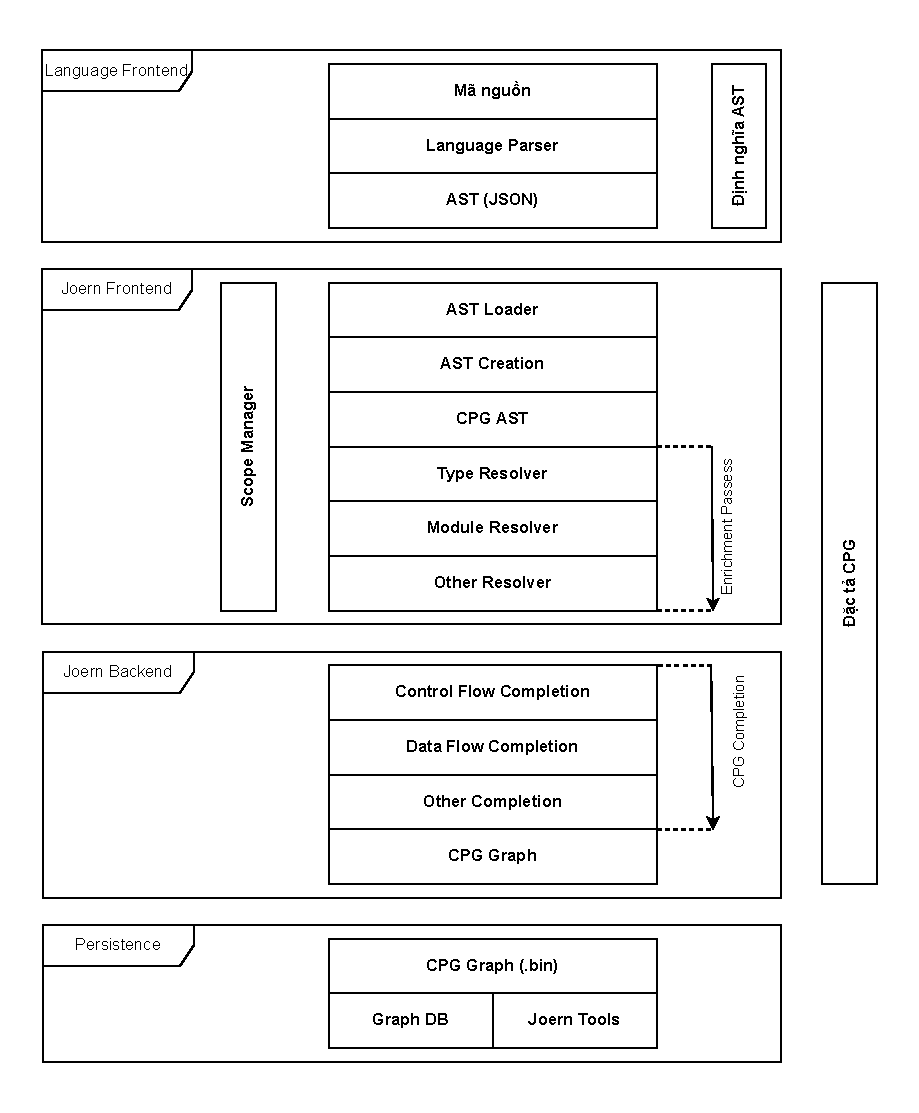
\includegraphics[width=1\columnwidth]{figures/c3/c3_arch.drawio.pdf}
	\centering
	\caption{Kiến trúc công cụ.}
	\label{img:c3_arch}
\end{figure}

Do sử dụng công cụ joern nên kiến trúc của công cơ về cơ bản sẽ là kiến trúc của Joern và mở rộng thêm. Phần này sẽ đi chi tiết hơn so với phần \ref{sec:joern_flow} đã trình bày ở phía trên. Các thành phần chính của công cụ bao gồm:

\textbf{Language Frontend} là phần đặc thù của mỗi ngôn ngữ lập trình, người dùng cần tự đảm nhiệm phần này khi muốn mở rộng công cụ Joern cho ngôn ngữ lập trình mới. Nhiệm vụ của Language Frontend là chuyển đổi mã nguồn thành cây AST dựa trên định nghĩa AST của đặc tả ngôn ngữ. Language Frontend có thể được cài đặt bằng bất cứ ngôn ngữ nào, do đó để có thể chuyển tiếp dư liệu cho quá trình tiếp theo, Language Frontend cần xuất cây AST ra dữ liệu trung gian, ở đây là JSON.

\textbf{Joern Frontend} là nơi chính thực hiện các công việc chuyển đổi cây AST của một ngôn ngữ lập trình cụ thể thành cây CPG theo đặc tả CPG. Đặc tả CPG sẽ được sử dụng xuyên suốt trong cả Joern Frontend và Joern Backend.
Joern Frontend sẽ nhận dữ liệu từ Language Frontend dưới dạng JSON bằng AST Loader. Cây AST sau khi được nạp vào Joern Frontend dưới ngôn ngữ Scala thì sẽ được chuyển đổi thành cây CPG bởi AST Creation. AST Creation thực hiện ánh xạ mỗi một loại nút AST của ngôn ng
sang một loại nút CPG tương ứng. Không chỉ tạo nút, AST Creation còn tạo các cạnh giữa các nút, giữa các nút có thể có nhiều cạnh, mỗi cạnh thể hiện một mối quan hệ giữa các nút. Mặc định giữa các nút có mối quan hệ là cạnh \textit{AST}. Tùy vào thể loại nút thì sẽ có các cạnh thể hiện mối quan hệ khác, ví dụ nút IF sẽ có cạnh \textit{CONDITION} nối với nút thể hiện điều kiện của IF.

\textbf{Scope Manager} được sử dụng trong Joern Frontend để thực hiện quản lý phạm vi của các biến, hàm hay các khai báo khác. Trong phần lớn các ngôn ngữ, một đơn vị cấu trúc sẽ có định danh riêng và định danh đó chỉ hợp lệ trong 1 giới hạn nhất định. Trong quá trình duyệt cây AST, Scope Manager sẽ kiểm soát thông tin về các định danh và phạm vi hoạt động của chúng. Khi sử dụng một định danh hoặc khai báo một định danh mới, Scope Manager sẽ kiểm tra xem khai báo đó có hợp lệ trong phạm vi hay không. Với Scope Manager ta có thể xác định được quan hệ giữa việc khai báo và sử dụng một biến, hàm hay đơn vị cấu trúc khác, từ đó có thể xác định được các cạnh giữa các nút trong cây CPG. Các cạnh sau này sẽ được sử dụng để xây dựng đồ thị CFG và PDG.

\textbf{Pass.} Như đã đề cập ở trên, một phần của cây AST CPG bao gồm các nút và cạnh đã được xây dựng ở AST Creation kết hợp với Scope Manager. Sau đó cây AST CPG sẽ tiếp tục được làm giàu thông tin bằng cách đi qua các Pass. Mỗi Pass sẽ bổ sung một lớp thông tin riêng biệt, ví dụ thông tin về kiểu dữ liệu, cấu trúc module, thứ tự thực hiện câu lệnh, ... Các lớp thông tin này hoàn toàn phụ thuộc vào ngữ cảnh của ngôn ngữ, do vậy số lượng pass cũng sẽ không cố định. Các pass thao tác trên AST CPG nên có thể dùng chung cho nhiều ngôn ngữ, nhưng cũng có các pass được xây dựng riêng cho đặc điểm của một ngôn ngữ cụ thể. Một pass có thể phụ thuộc vào kết quả của pass trước đó hoặc chạy độc lập nên thứ tự chạy các pass cũng rất quan trọng. Ở đây, công cụ chỉ sử dụng 2 pass là Type Resolver và Module Resolver để xử lý kiểu dữ liệu và hệ thống module của Rust, các pass khác sẽ được xây dựng trong tương lai. Sau khi chạy qua các pass, cây AST CPG đã được bổ sung các lớp thông tin nhất định và đây cũng là công đoạn cuối cùng của Joern Frontend.

\textbf{Joern Backend}. Khi chuyển đổi một ngôn ngữ sang CPG, người dùng phải tự thực hiện công đoạn Language Frontend và Joern Frontend để xây dựng cây CPG. Các thông tin có được từ 2 bước trên sẽ được Joern Backend sử dụng để tự động hoàn thiện cây AST CPG thành đồ thị CPG. Các nút, cạnh mới về luồng điều khiển, luồng dữ liệu sẽ được thêm vào và kết nối với các cạnh, nút đã tồn tại. Không chỉ lớp thông tin về điều khiển và dữ liệu, Joern Backend bổ sung các lớp thông tin như  FileSystem, CallGraph, Shortcuts, TagsAndLocation, Annotation \cite{joernCodeProperty}. Kết quả cuối cùng của Joern Backend là một đồ thị CPG hoàn chỉnh.

\textbf{Persistence}. Đồ thị CPG có thể được lưu trư bền vững dưới dạng file nhị phân. File này có thể tiếp tục được chuyển đổi thành kiểu dữ liệu tương thích với các công cụ khác như Neo4j để thực hiện các truy vấn phức tạp hơn, hoặc sử dụng bằng các công cụ khác của Joern.


% \section{Xây dựng cây cú pháp trừu tượng}

% \section{Xây dựng đồ thị thuộc tính mã nguồn (CPG)}